\documentclass{../exhibit}

\title{Pi-rate Walk}

%% Font
\usepackage{imfellEnglish}
\usepackage[T1]{fontenc}
\raggedright

\usepackage{background}

\backgroundsetup{
scale=1,
color=black,
opacity=0.4,
angle=0,
contents={%
  \includegraphics[height=\paperheight]{mapBackground.jpg}%%https://upload.wikimedia.org/wikipedia/commons/8/81/Nautical_chart_of_the_West_Indies_1797.jpg
  }%
}




%% For the context
%% https://tex.stackexchange.com/questions/86150/torn-page-effect/86151#86151
\usepackage{tikz}
\usetikzlibrary{decorations.pathmorphing}
\definecolor{paper}{RGB}{239,227,157}





\renewcommand{\maketitle}{ %
  \begin{center}
    \scalebox{8}{\thetitle}
  \end{center}
  
\begin{tabular*}{\textwidth}{c @{\extracolsep{\fill}} c}  
\resizebox{4in}{!}{\begin{minipage}[b]{3in}\huge\directions\end{minipage}} &
  \resizebox{4in}{!}{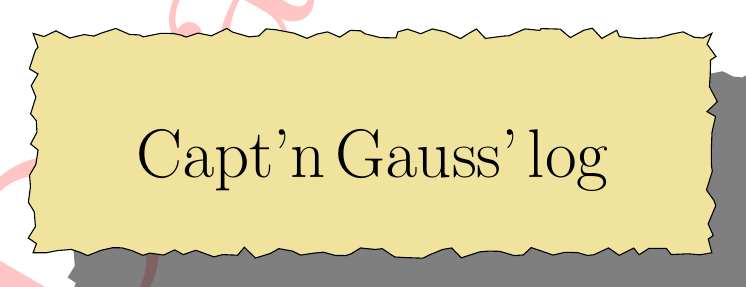
\begin{tikzpicture}[pencildraw/.style={ %
    decorate,
    decoration={random steps,segment length=4pt,amplitude=2pt}
    } %
]
\node[
preaction={fill=black,opacity=.5,transform canvas={xshift=.5cm,yshift=-.5cm}},
pencildraw,draw,fill=paper,text width=3in,inner sep=.5cm] 
{\begin{center}\Huge Capt'n Gauss' log \end{center}\vspace{.7cm} {\huge\context}};
\end{tikzpicture}}

\end{tabular*}

\vfill

\includegraphics[width=3in]{logoPirate.png}\hfill \includegraphics[width=2in]{bammLogo.png}


}


\begin{document}



\begin{context}
  The first ten digits of $\pi$ be:

  \[
  \pi=3.141592653\dots
  \]

  Like a true $\pi$-rate, we place them in a circle and dance around!


  When the music stops, if yer number be called,



  THE

  \qquad TREASURE

  
  \qquad \qquad \qquad  IS YOURS!
\end{context}



\begin{directions}

  Write the first 10 digits of $\pi$ on the ground in a circle.
  \begin{itemize}
    \item Walk around to music,
    \item when the music stops,
    \item stop at a number.
    \item If your number is chosen, you win!
  \end{itemize}
  \end{directions}



\begin{example}\HUGE
  \begin{center}
  \begin{tikzpicture}[scale=2.5]
    \node at ({2*sin(0*360/10)},{2*cos(0*360/10)}) {3.};
    \node at ({2*sin(1*360/10)},{2*cos(1*360/10)}) {1};
    \node at ({2*sin(2*360/10)},{2*cos(2*360/10)}) {4 };
    \node at ({2*sin(3*360/10)},{2*cos(3*360/10)}) {1 };
    \node at ({2*sin(4*360/10)},{2*cos(4*360/10)}) {5 };
    \node at ({2*sin(5*360/10)},{2*cos(5*360/10)}) {9 };
    \node at ({2*sin(6*360/10)},{2*cos(6*360/10)}) {2 };
    \node at ({2*sin(7*360/10)},{2*cos(7*360/10)}) {6 };
    \node at ({2*sin(8*360/10)},{2*cos(8*360/10)}) {5 };
    \node at ({2*sin(9*360/10)},{2*cos(9*360/10)}) {3\dots};

    \node at (0,0) {\scalebox{3}{$\pi$}};
  \end{tikzpicture}
  \end{center}
\end{example}



\begin{mathConnections}
  https://bartsnapp.github.io/Math-Outreach-Exhibits/template/
\end{mathConnections}
\end{document}
